\documentclass{beamer}
\mode<presentation>
\usetheme{CambridgeUS}
\usepackage[russian]{babel}
\usepackage[utf8]{inputenc}
\usepackage[T2A]{fontenc}
\usepackage{sansmathaccent}

\usepackage{verbatim}
\usepackage{alltt}

\pdfmapfile{+sansmathaccent.map}
\title[Software Design]{Основы объектно-ориентированного программирования}
\author{Наумов Д.А., доц. каф. КТ}
\date[16.09.2019] {Основы программной инженерии, 2019}

\begin{document}

%ТИТУЛЬНЫЙ СЛАЙД
\begin{frame}
  \titlepage
\end{frame}
  
%СОДЕРЖАНИЕ ЛЕКЦИИ
\begin{frame}
  \frametitle{Содержание лекции}
  \tableofcontents  
\end{frame}
  
\section{Развитие языков как абстрактных моделей}

\subsection{Концепции проектирования и языки программирования}

\begin{frame}
\begin{block}{Объектно-ориентированное программирование (ООП)}
самая распространенная в современной проектной практике парадигма программирования. 
\end{block}
\begin{itemize}
\item поддерживается большинством современных языков программирования;
\item реализации концепций и механизмов ООП могут отличаться в разных языках.
\end{itemize}
Широкое применение технологии = технология позволяет успешно решать актуальные проблемы проектирования.
\end{frame}

\begin{frame}[t]{Прогресс информационных технологий}
\begin{figure}[h]
\centering
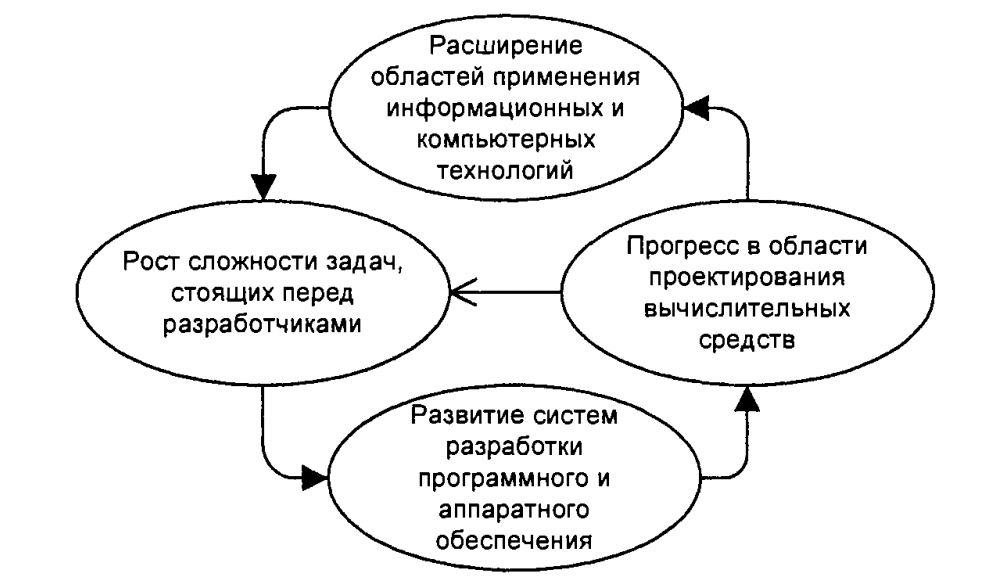
\includegraphics[scale=0.25]{images/lec04-pic01.png}
\end{figure}
\begin{itemize}
\item качество проектирования <- квалификация и способности проектировщиков;
\item технология проектирования помогает построить качественный продукт;
\item необходимо изучать не языки программирования сами по себе, а концепции, выражаемые этими языками.
\end{itemize}
\end{frame}

\subsection{Абстрактные модели, лежащие в основе языков программирования}
\begin{frame}
\begin{block}{Язык программирования}
модель (виртуальная вычислительная машина), позволяющая наиболее эффективно использовать возможности вычислительных средств, существенные для конкретных областей применения. 
\end{block}
\begin{itemize}
\item при написании программ ориентируются не на вычислительную машину как таковую, а на некоторую абстрактную модель вычислительного устройства;
\item качество модели определяет качество
и эффективность проектирования;
\item сложность задач, которые возможно решить, непосредственно связана с уровнем абстракции как при постановке задачи, так и в ходе ее решения.
\end{itemize}
\begin{block}{Развитие языков программирования}
это, прежде всего, развитие абстрактных моделей, облегчающих и систематизирующих проектирование.
\end{block}
\end{frame}

\begin{frame}
\begin{block}{Методология структурного императивного программирования}
воплощает подход, характеризующийся принципом последовательного изменения состояния вычислителя пошаговым образом с поддержкой концепции структурного программирования. 
\end{block}
\begin{itemize}
\item ориантируется на класс архитектур фон Неймана;
\item примеры языков: Fortran, Pascal, С, PL/1.
\end{itemize}
Развитие структурного программирования:
\begin{itemize}
\item функционально-иерархическая декомпозиция;
\item структурная организация данных;
\item повторное использование проектных решений;
\item технология тестирования программного обеспечения.
\end{itemize}
\end{frame}

\begin{frame}
Проблема процедурных языков:
\begin{itemize}
\item уровень абстракции все еще требует от программиста мышления в большей мере в терминах вычислительной машины;
\item качество проектирования определяется в итоге тем, насколько удачно программисту удалось установить соответствие между пространством понятий, характерных для решаемой задачи, и набором изобразительных средств языка;
\item абстрагирование, достигаемое посредством использования процедур, хорошо
подходит для описания абстрактных действий, но не предоставляет адекватных языковых средств для описания абстрактных объектов.
\end{itemize}
Альтернативные модели:
\begin{itemize}
\item функциональное программирование, язык LISP: все задачи, в конечном счете, могут быть сведены к работе со списками;
\item логическое программирование, язык Prolog: все задачи могут быть сведены к цепочке логических рассуждений.
\end{itemize}
\end{frame}

\subsection{Сущность объектно-ориентированного подхода}

\begin{frame}[t]
ООП предоставляет разработчику инструмент, который позволяет описать задачу и существенную часть реализации проекта в терминах, характеризующих предметную область, а не компьютерную модель. 
\begin{figure}[h]
\centering
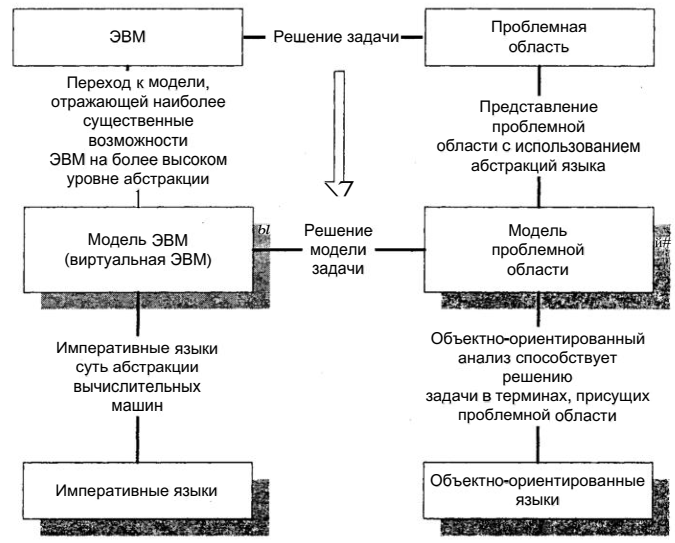
\includegraphics[scale=0.4]{images/lec04-pic02.png}
\end{figure}
ООП предоставляет разработчикам гибкий мощный универсальный инструмент, не связанный с каким-то определенным классом задач.
\end{frame}

\begin{frame}[t]
\begin{figure}[h]
\centering
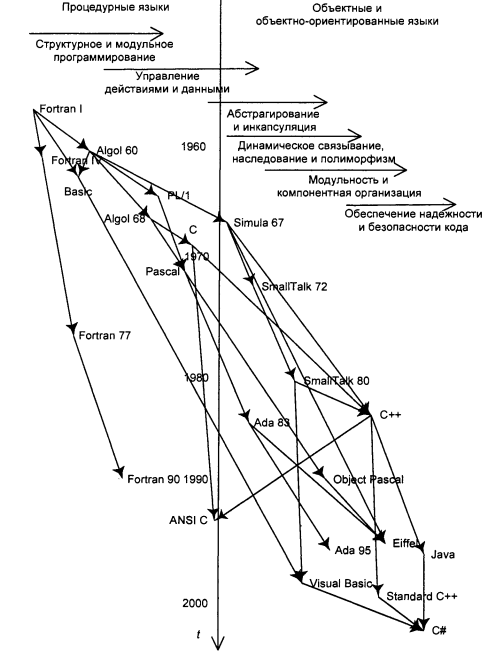
\includegraphics[scale=0.5]{images/lec04-pic03.png}
\end{figure}
\end{frame}

\begin{frame}
\begin{itemize}
\item объектно-ориентированное программирование улучшает проектирование, фокусируясь на данных как более стабильном элементе вычислительной системы; 
\item объектно-ориентированный подход концентрируется на разработке кода, направленного на повторное использование;
\item объектно-ориентированная модель обеспечивает лучшую масштабируемость проектов;
\item большинство успешных современных технологий
проектирования программных систем предполагает преимущественное или
искчючительное использование объектно-ориентированной парадигмы.
\end{itemize}
\end{frame}

\section{Элементы объектной модели}
\begin{frame}
Объектную модель составляют четыре главных элемента:
\begin{itemize}
\item абстрагирование (abstraction);
\item инкапсуляция (encapsulation);
\item модульность (modularity);
\item иерархия (hierarchy).
\end{itemize}
\begin{block}{Абстрагирование}
позволяет выделить существенные характеристики некоторого объекта, отличающие его от всех других видов объектов. Абстракция четко определяет концептуальные границы объекта с точки зрения наблюдателя.
\end{block}
\begin{block}{Инкапсуляция}
это процесс отделения друг от друга элементов объекта, определяющих его устройство и поведение; инкапсуляция также служит для того, чтобы изолировать внешнее поведение объекта от его внутреннего устройства.
\end{block}
\end{frame}

\begin{frame}
Объектную модель составляют четыре главных элемента:
\begin{itemize}
\item абстрагирование (abstraction);
\item инкапсуляция (encapsulation);
\item модульность (modularity);
\item иерархия (hierarchy).
\end{itemize}
\begin{block}{Иерархия}
это упорядочение абстракций, средство классификации объектов, систематизация связей между объектами.
\end{block}
\begin{block}{Модульность}
это представление системы в виде совокупности обособленных сегментов, связь между которыми обеспечивается посредством связей между классами, определяемыми в этих сегментах.
\end{block}
\end{frame}

\begin{frame}{Абстракция}
\begin{block}{Абстракция}
выделяет существенные характеристики некоторого объекта, отличающие его от всех других видов объектов и, таким образом, четко определяет его концептуальные границы с точки зрения наблюдателя.
\end{block}
Два вида абстракций в ООП:
\begin{itemize}
\item \textbf{тип данных объектной природы (класс)}— определяемое программистом
расширение исходных типов языка;
\item \textbf{экземпляр класса (объект)} — переменная класса. Объект обладает состоянием, поведением и идентичностью.
\end{itemize}
Состояние объекта:
\begin{itemize}
\item характеризуется набором его свойств (атрибутов) и текущими значениями каждого из этих свойств;
\item результат его поведения
\end{itemize}
\end{frame}

\begin{frame}[t]
\begin{figure}[h]
\centering
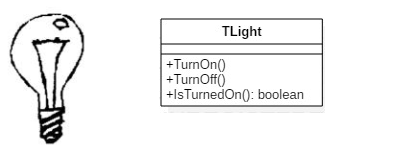
\includegraphics[scale=0.75]{images/lec04-pic04.png}
\end{figure}
\begin{figure}[h]
\centering
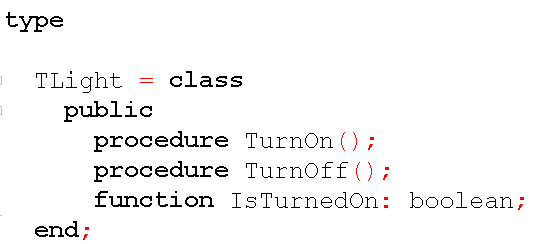
\includegraphics[scale=0.75]{images/lec04-pic05.png}
\end{figure}
\end{frame}

\begin{frame}[t]
Описание и создание экземпляра класса:
\begin{figure}[h]
\centering
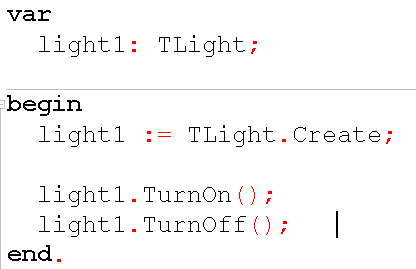
\includegraphics[scale=0.6]{images/lec04-pic06.png}
\end{figure}
\begin{itemize}
\item объектная переменная хранит информацию, характеризующую объект;
\item объект размещается в динамической памяти (Create).
\end{itemize}
\textbf{Абстрагирование направлено на наблюдаемое поведение объекта (а не на внутреннюю реализацию).}
\end{frame}

\begin{frame}{Инкапсуляция}
\begin{block}{Инкапсуляция}
изолирует интерфейс от реализации и связана с управлением доступом к данным класса.
\end{block}
\begin{figure}[h]
\centering
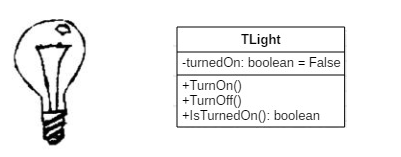
\includegraphics[scale=0.5]{images/lec04-pic07.png}
\end{figure}
\begin{figure}[h]
\centering
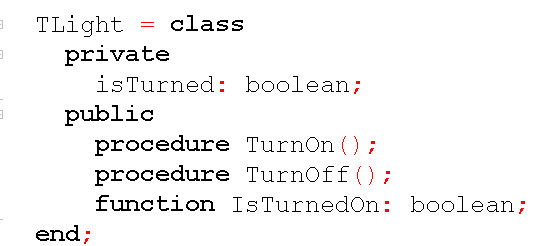
\includegraphics[scale=0.5]{images/lec04-pic08.png}
\end{figure}
\end{frame}

\begin{frame}{Инкапсуляция}
Инкапсуляция предполагает возможность ограничения доступа к данным класса из 
других классов. 
\begin{itemize}
\item это позволяет упростить интерфейс класса, показав наиболее существенные для внешнего пользователя данные и методы;
\item скрытие реализации обеспечивает возможность внесения изменений в реализацию класса без изменения других классов.
\end{itemize}
\begin{figure}[h]
\centering
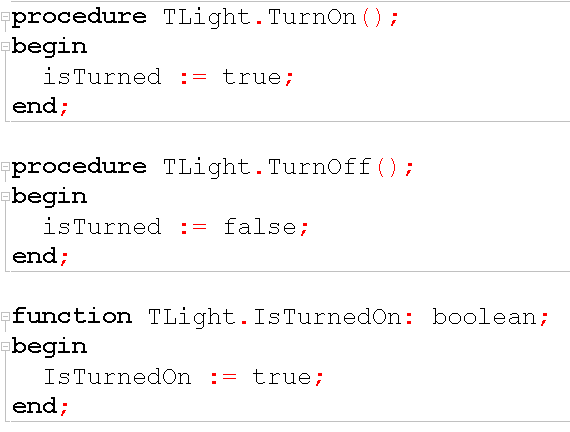
\includegraphics[scale=0.3]{images/lec04-pic09.png}
\end{figure}
\textbf{Доступ к закрытым данным возможен из всех классов, расположенных в том же модуле, что и анализируемый класс.}
\end{frame}

\begin{frame}{Отношения классов}
\begin{itemize}
\item \textbf{Отношение обобщения} (generalization) описывает отношение между общей
сущностью и ее конкретным воплощением (один класс является специализацией другого класса);
\item \textbf{Отношение ассоциации} (association) описывает структурное отношение,
показывающее, что объекты одного типа некоторым образом связаны
с объектами другого типа (находятся в отношении типа "часть/целое").
\item \textbf{Отношение зависимости} (dependency) описывает отношение использования, при котором изменение в спецификации одного класса может повлиять на класс, его использующий (объекты некоторого класса передаются в качестве аргументов функциям-членам другого класса).
\item \textbf{Отношение реализации} (realization) - семантическое отношение, при котором класс гарантирует выполнение контракта, определяемого некоторым интерфейсом.
\end{itemize}
\end{frame}

\begin{frame}{Отношение обощения}
\begin{figure}[h]
\centering
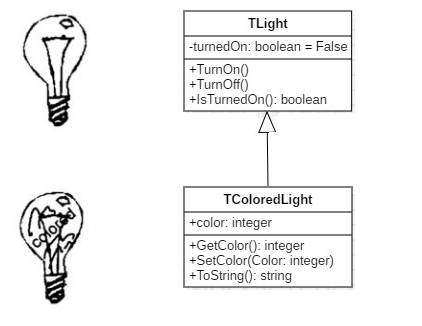
\includegraphics[scale=0.75]{images/lec04-pic10.png}
\end{figure}
\end{frame}

\begin{frame}{Отношение обощения}
\begin{figure}[h]
\centering
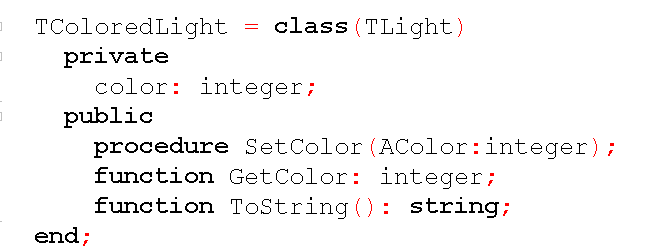
\includegraphics[scale=0.7]{images/lec04-pic11.png}
\end{figure}
\end{frame}

\begin{frame}{Отношение обощения}
\begin{figure}[h]
\centering
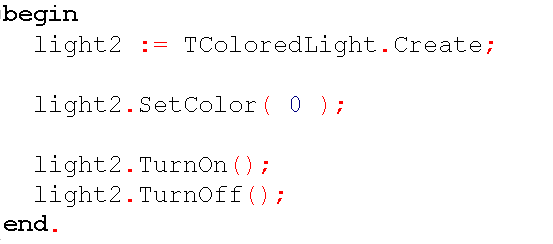
\includegraphics[scale=0.75]{images/lec04-pic12.png}
\end{figure}
\end{frame}

\begin{frame}{Подобъект базового класса}
\begin{figure}[h]
\centering
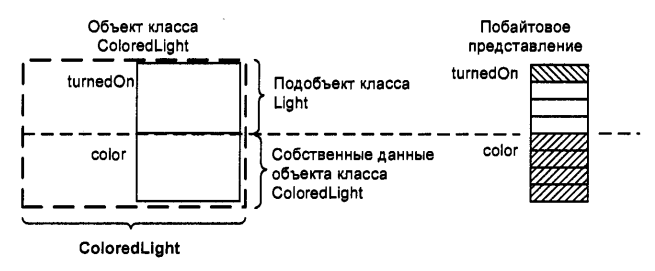
\includegraphics[scale=0.7]{images/lec04-pic13.png}
\end{figure}
\end{frame}

\begin{frame}{Отношение ассоциации}
\begin{figure}[h]
\centering
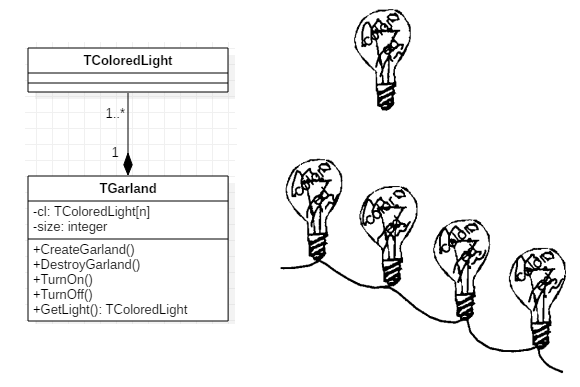
\includegraphics[scale=0.75]{images/lec04-pic14.png}
\end{figure}
\end{frame}

\begin{frame}{Отношение ассоциации}
\begin{figure}[h]
\centering
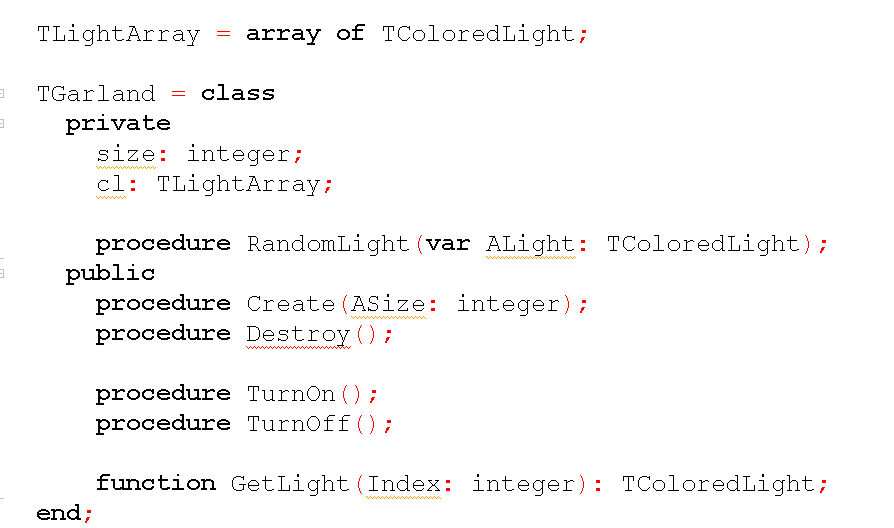
\includegraphics[scale=0.5]{images/lec04-pic15.png}
\end{figure}
\end{frame}

\begin{frame}{Размещение объектов в памяти}
\begin{figure}[h]
\centering
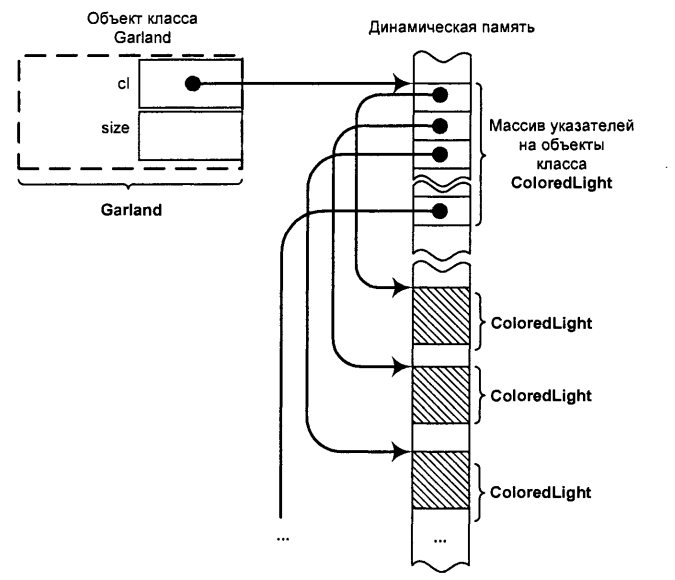
\includegraphics[scale=0.5]{images/lec04-pic16.png}
\end{figure}
\end{frame}

\begin{frame}{Пример}
\begin{figure}[h]
\centering
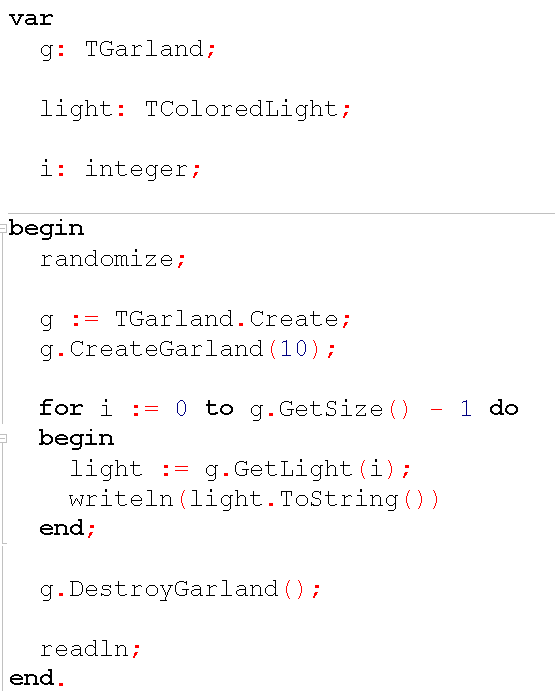
\includegraphics[scale=0.5]{images/lec04-pic17.png}
\end{figure}
\end{frame}

\begin{frame}{Отношение зависимости}
\begin{block}{Отношение зависимости}
является таким типом отношений между классами, когда изменение в спецификации или реализации одного класса влияет на спецификацию или реализацию другого класса.
\end{block}
\begin{figure}[h]
\centering
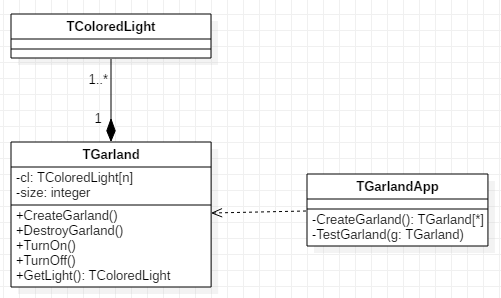
\includegraphics[scale=0.6]{images/lec04-pic18.png}
\end{figure}
\end{frame}

\begin{frame}{Отношение реализации}
\begin{block}{Отношение реализации}
используется для определения отношения между интерфейсом и классом, реализующим интерфейс.
\end{block}
Интерфейс определяет набор элементов (как правило, действий), характерных для объектов, обладающих определенными свойствами.
\begin{figure}[h]
\centering
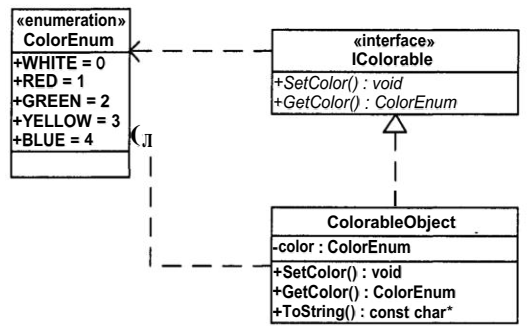
\includegraphics[scale=0.6]{images/lec04-pic19.png}
\end{figure}
\end{frame}

\begin{frame}{Отношение реализации}
Наличие интерфейсов предоставляет возможность работать с объектами разных типов в той части, которая поддерживает соответствующий интерфейс.
\begin{figure}[h]
\centering
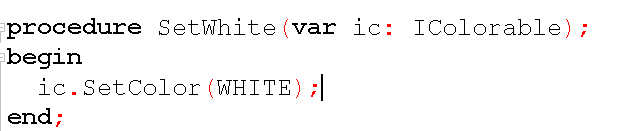
\includegraphics[scale=0.75]{images/lec04-pic20.png}
\end{figure}
\end{frame}

\begin{frame}
\begin{figure}[h]
\centering
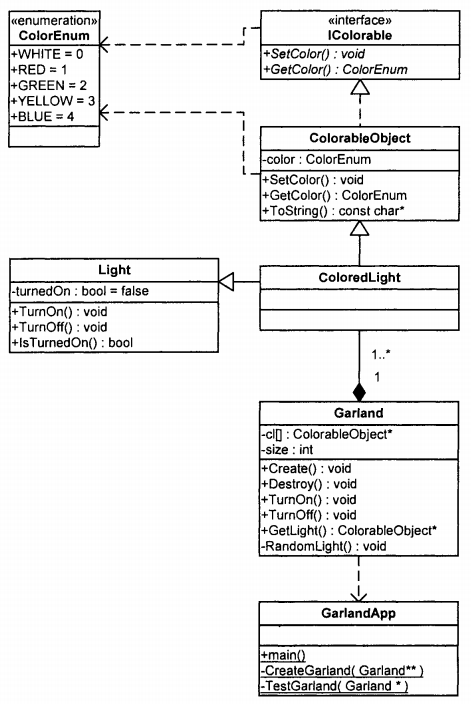
\includegraphics[scale=0.45]{images/lec04-pic21.png}
\end{figure}
\end{frame}

\begin{frame}{Типы структурных иерархий}
Иерархическая декомпозиция и иерархическая организация ПО образуют один из основных систематических методов преодоления сложности программного обеспечения.
\begin{itemize}
\item cтруктурная иерархия "is-part-of" (агрегирование как разновидность ассоциации)
\item Структурные иерархии "is-а" и "is-like-a"
\end{itemize}
\begin{block}{Обобщение}
означает, что объекты классапотомка могут использоваться везде, где допустимы объекты родительского класса. 
\end{block}
\end{frame}

\begin{frame}
\begin{itemize}
\item Создавая базовый тип (базовый класс), программист выражает наиболее общие идеи относительно объектов, из которых конструируется программа.
\item В производных классах программист уточняет различия в реализации конструкций базового класса.
\item Производный класс полностью дублирует интерфейс базового класса, т. е. дублирует наблюдаемое поведение объекта базового класса. 
\end{itemize}
\begin{figure}[h]
\centering
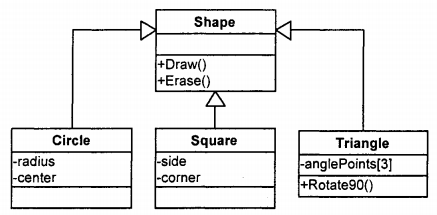
\includegraphics[scale=0.7]{images/lec04-pic22.png}
\end{figure}
\end{frame}

\begin{frame}
Поведение объекта производного класса может отличаться от поведения объекта базового класса.
\begin{figure}[h]
\centering
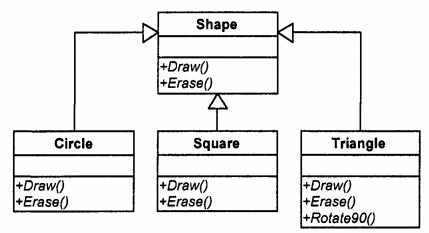
\includegraphics[scale=0.6]{images/lec04-pic23.png}
\end{figure}
\begin{itemize}
\item может потребоваться изменение реализации уже существующих методов; (рис.
\item дочерний класс предоставляет операции, замещающие операции родителя с такой же сигнатурой ("is-like-a")
\end{itemize}
\begin{block}{Замещение (перекрытие, overriding) метода класса}
механизм изменения реализации метода класса с сохранением интерфейса, определяемого базовым классом.
\end{block}
\end{frame}

\begin{frame}{Полиморфизм}
Поведение объектов, на которых вызываются видоизмененные методы, интерфейс к которым заявлен в базовом классе, называют \textbf{полиморфным}, а механизм, обеспечивающий такое поведение, называют \textbf{полиморфизмом}.

Мы имеем возможность:
\begin{itemize}
\item работая с объектами разных типов, представляющих различные абстракции, мы можем использовать методы, которые имеют одинаковый интерфейс, что, в конечном счете, упрощает и реализацию программы, и ее восприятие;
\item разрабатывать общие процедуры обработки объектов.
\end{itemize}
\end{frame}

\end{document}
